\documentclass[UTF8]{article} 
\usepackage{graphicx}
\usepackage{subfigure}
\usepackage{amsmath}
\usepackage{makecell}
\usepackage[utf8]{inputenc}
\usepackage[space]{ctex} %中文包
\usepackage{listings} %放代码
\usepackage{xcolor} %代码着色宏包
\usepackage{CJK} %显示中文宏包
\usepackage{float}


\definecolor{mygreen}{rgb}{0,0.6,0}
\definecolor{mygray}{rgb}{0.5,0.5,0.5}
\definecolor{mymauve}{rgb}{0.58,0,0.82}
\lstset{
	backgroundcolor=\color{white}, 
	basicstyle = \footnotesize,       
	breakatwhitespace = false,        
	breaklines = true,                 
	captionpos = b,                    
	commentstyle = \color{mygreen}\bfseries,
	extendedchars = false,             
	frame =shadowbox, 
	framerule=0.5pt,
	keepspaces=true,
	keywordstyle=\color{blue}\bfseries, % keyword style
	language = Verilog,                     % the language of code
	otherkeywords={string}, 
	numbers=left, 
	numbersep=5pt,
	numberstyle=\tiny\color{mygray},
	rulecolor=\color{black},         
	showspaces=false,  
	showstringspaces=false, 
	showtabs=false,    
	stepnumber=1,         
	stringstyle=\color{mymauve},        % string literal style
	tabsize=4,          
	title=\lstname                      
}


\title{中国科学技术大学计算机学院\\《数字电路实验》报告}
\author{}

\date{}

\begin{document}
	\maketitle
	\begin{figure}[H]
		\centering
		
\includegraphics[width=2.5in]{xiaohui.jpg}\vspace{0.5cm}\\
		\large{
			实验题目:简单时序逻辑电路\\
			学生姓名:王章瀚\\
			学生学号:PB18111697\\
			完成日期:2019/10/20\\
		}\vspace{2cm}
		
		\large{计算机实验教学中心制\\2019年09月\\}
		\thispagestyle{empty}
		\clearpage  % 清除当页页码
	\end{figure}


	\section{实验目的}
	掌握时序逻辑相关器件的原理及底层结构\par
	能够用基本逻辑门搭建各类时序逻辑器件\par
	能够使用 Verilog HDL 设计简单逻辑电路\par
	
	\section{实验环境}
	PC 一台\par
	Windows 或 Linux 操作系统\par
	Java 运行环境(jre)\par
	Logisim 仿真工具\par
	vlab.ustc.edu.cn (jre 和 Logisim 工具都可在此网站获取)\par
	
	\section{实验过程}
	\subsection{搭建双稳态电路}
	此处值得注意的是,在 Logisim 中搭建此电路时,应先将两条交叉耦合线断开一条,等输入信号将其状态初始到确定状态后再将耦合线连上。否则电路将处于一种不确定状态。\par
	\begin{figure}[H]
		\begin{minipage}[H]{0.45\linewidth}
			\centering
			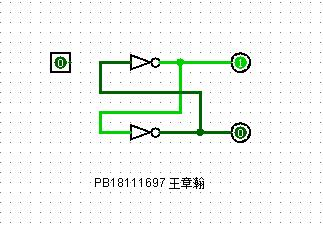
\includegraphics[scale=0.7]{1_1.jpg}
			\label{1_1}
		\end{minipage}
		\begin{minipage}[H]{0.45\linewidth}
			\centering
			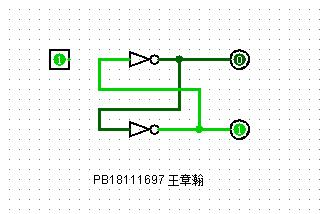
\includegraphics[scale=0.7]{1_2.jpg}
			\label{1_2}
		\end{minipage}\\
		\begin{center}
			\begin{minipage}[H]{0.5\linewidth}
				\centering
				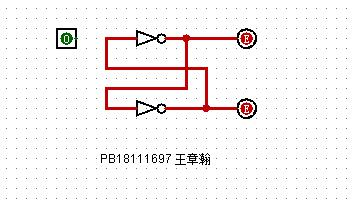
\includegraphics[scale=0.7]{1_3.jpg}
				\label{1_3}
			\end{minipage}
		\end{center}
	\end{figure}


	\subsection{搭建 SR 锁存器}
	由于刚才搭建的双稳态电路没有输入信号,无法进行操作。故将两非门用或非门代替。输入信号为S和R,输出信号为Q和/Q(用以表示$\overline{Q}$)。如下四图所示:
	
	\begin{figure}[H]
		\begin{minipage}[H]{0.49\linewidth}
			\centering
			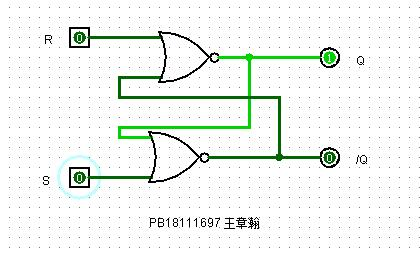
\includegraphics[width=1\linewidth]{2_00.jpg}
			\label{2_00}
		\end{minipage}
		\begin{minipage}[H]{0.49\linewidth}
			\centering
			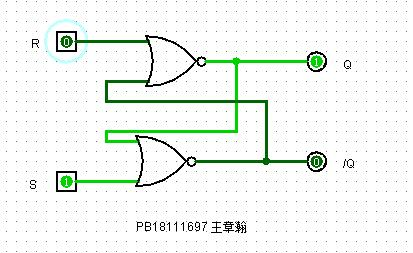
\includegraphics[width=1\linewidth]{2_01.jpg}
			\label{2_01}
		\end{minipage}\\
		\begin{minipage}[H]{0.49\linewidth}
			\centering
			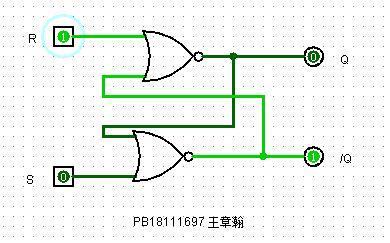
\includegraphics[width=1\linewidth]{2_10.jpg}
			\label{2_10}
		\end{minipage}
		\begin{minipage}[H]{0.49\linewidth}
			\centering
			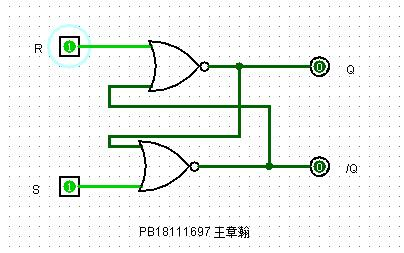
\includegraphics[width=1\linewidth]{2_11.jpg}
			\label{2_11}
		\end{minipage}
	\end{figure}


	\subsection{搭建 D 锁存器}
	前面的SR锁存器中,两个输入为1是一种未定义状态,我们不希望它出现。为此在SR锁存器前面添加两个与门和一个非门。如下图:
	
	\begin{figure}[H]
		\centering
		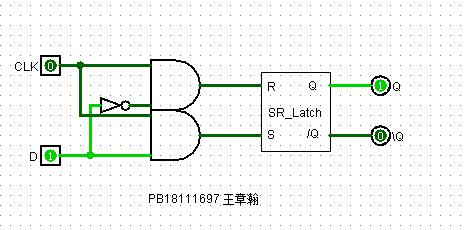
\includegraphics[width=1\linewidth]{D_Latch.jpg}
		\label{D_Latch}
	\end{figure}
	只有CLK为高电平时,锁存器的值才会随D变化,如下图:
	
	\begin{figure}[H]
		跟随:
		\begin{minipage}[H]{0.49\linewidth}
			\centering
			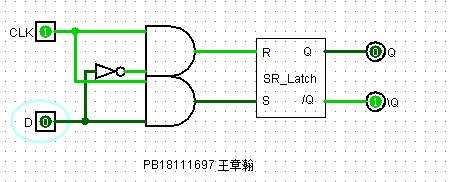
\includegraphics[width=1\linewidth]{D_Latch_Follow_0.jpg}
			\label{D_Latch_Follow_0}
		\end{minipage}
		\begin{minipage}[H]{0.49\linewidth}
			\centering
			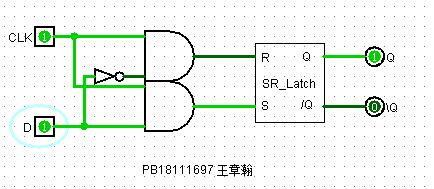
\includegraphics[width=1\linewidth]{D_Latch_Follow_1.jpg}
			\label{D_Latch_Follow_1}
		\end{minipage}\\
		锁存:
		\begin{minipage}[H]{0.49\linewidth}
			\centering
			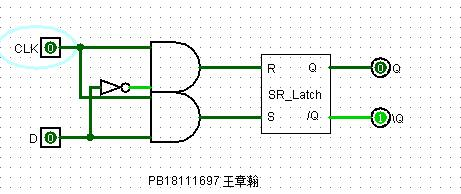
\includegraphics[width=1\linewidth]{D_Latch_Lock_0.jpg}
			\label{D_Latch_Lock_0}
		\end{minipage}
		\begin{minipage}[H]{0.49\linewidth}
			\centering
			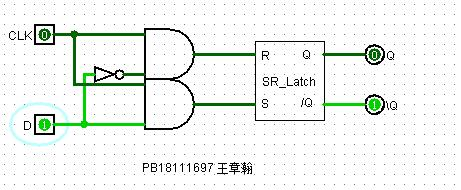
\includegraphics[width=1\linewidth]{D_Latch_Lock_1.jpg}
			\label{D_Latch_Lock_1}
		\end{minipage}\\
	\end{figure}



	\subsection{搭建 D 触发器}
	如果我们将两个 D 锁存器串起来,其控制信号有效值始终相反,实际上这就构成了触发器。\par
	\begin{figure}[H]
		\centering
		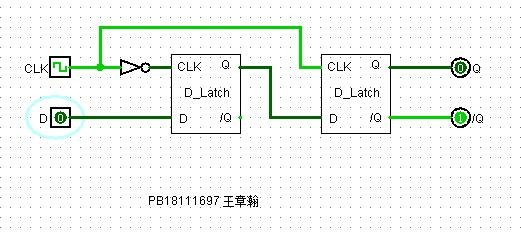
\includegraphics[width=1\linewidth]{D_FF.jpg}
		\label{D_FF}
	\end{figure}
	利用Logisim的仿真功能,设置频率为1HZ,通过分析我们可以发现,只有在 CLK 信号由低电平变为高电平的瞬间, D 信号才会传播到 Q 端,其余时刻 Q 端的值都保持不变。\par
	写出该过程的代码,\par
	\begin{lstlisting}[language=Verilog]
	module D_FF(
		input clk,
		input d,
		output reg q
		);
		always @(posedge clk)
			q <= d;
	endmodule	
	\end{lstlisting}
	利用Vivado的仿真得到波形图,如下:
	\begin{figure}[H]
		\centering
		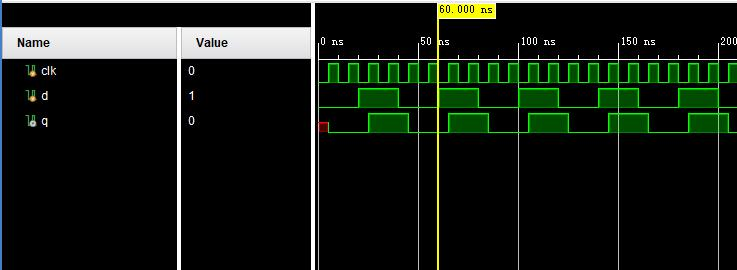
\includegraphics[width=1\linewidth]{D_FF_Oscillogram.jpg}
		\label{D_FF_Oscillogram}
	\end{figure}
	此外,我们还可以添加复位信号,当复位信号有效(低电平邮箱)时,输出信号Q始终为0,如下图:
	\begin{figure}[H]
		\centering
		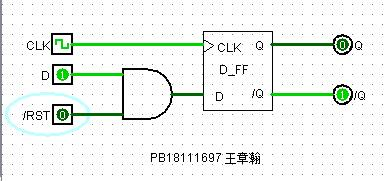
\includegraphics[width=1\linewidth]{D_FF_RST.jpg}
		\label{D_FF_RST}
	\end{figure}
	带复位信号的电路代码如下,\par
	\begin{lstlisting}[language=Verilog]
	module D_FF_RST(
		input clk,
		input d,
		input rst_n,
		output reg q
		);
		always@(posedge clk)
		begin
			if(rst_n==0)
				q <= 1'b0;
			else
				q <= d;
		end
	endmodule
	\end{lstlisting}
	波形图如下,
	\begin{figure}[H]
		\centering
		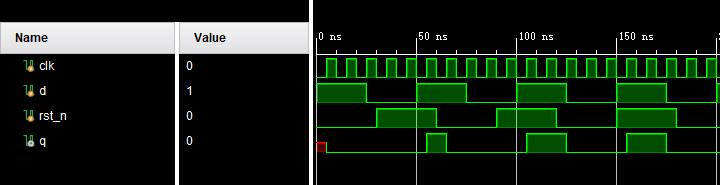
\includegraphics[width=1\linewidth]{D_FF_RST_Oscillogram.jpg}
		\label{D_FF_RST_Oscillogram}
	\end{figure}
	上述这种触发器的复位信号只有在时钟信号的上升沿才起作用,在非上升沿时刻,复位信号不起作用。这种复位方式称为同步复位。另外还有一种异步复位的方式,可以使得不论时钟和D信号如何,一旦复位信号有效,输出端 Q 立即变为确定的复位值。而异步复位与同步复位最大的区别在于,复位信号与时钟信号同时出现在了 always 语句的敏感变量列表中。其波形图如下:
	
	\begin{figure}[H]
		\centering
		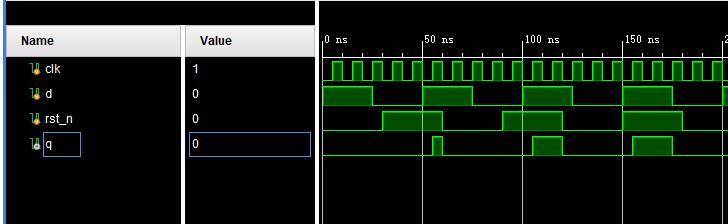
\includegraphics[width=1\linewidth]{D_FF_RST_Oscillogram_.jpg}
		\label{D_FF_RST_Oscillogram_}
	\end{figure}
	D触发器是一种边沿敏感器件,因此由D触发器为核心构成的电路一般称为同步时序逻辑电路,而锁存器构成的一般都是异步时序电路。\par
	
	
	\subsection{搭建寄存器}
	寄存器本质上就是触发器,如下图,用4个D触发器构成一个储存4bit数据的寄存器,并有低电平有有效的复位信号。
	\begin{figure}[H]
		\centering
		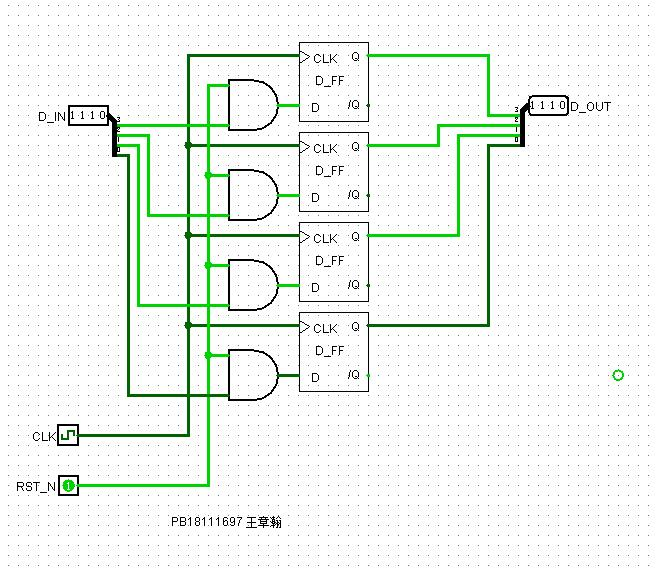
\includegraphics[width=1\linewidth]{step5_register.jpg}
		\label{step5_register}
	\end{figure}
	该寄存器的行为表现可以总结如下:若复位信号有效,则在时钟上升沿时,输出全部复位为0,否则在上升沿时,更新为输入D\_IN的值。\par
	其Verilog代码如下:\par
	\begin{lstlisting}[language=Verilog]
	module REG4(
		input CLK,
		input RST_N,
		input [3:0] D_IN,
		output reg [3:0] D_OUT
		);
		always @(posedge CLK)
		begin
			if(RST_N == 0)
				D_OUT <= 4'b0;
			else
				D_OUT <= D_IN;
		end
	endmodule
	\end{lstlisting}
	如要使复位信号将输出置为0011,其verilog代码实现显然。电路图实现可以如下:
	\begin{figure}[H]
		\centering
		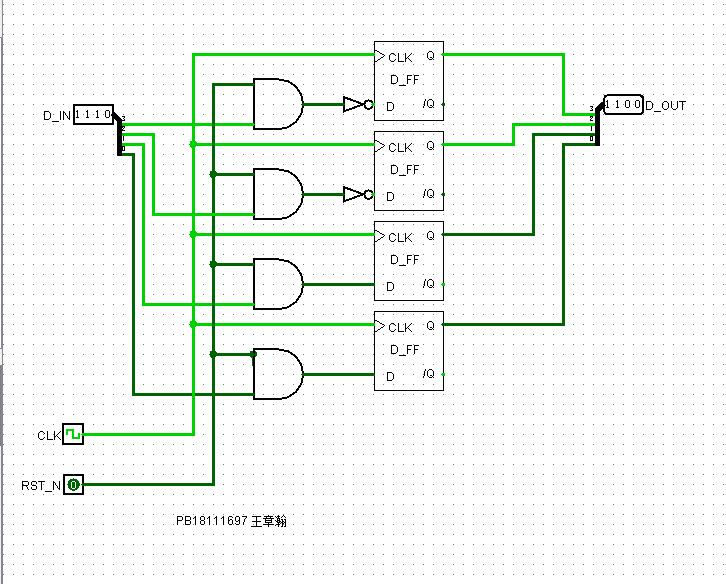
\includegraphics[width=1\linewidth]{step5_register_resetTo1100.jpg}
		\label{step5_register_resetTo1100}
	\end{figure}


	\subsection{搭建简单时序逻辑电路}
	我们利用 4bit 寄存器,搭建一个 4bit 的计数器,该计数器在 0~15之间循环计数,复位时输出值为 0,电路图如下所示:
	\begin{figure}[H]
		\centering
		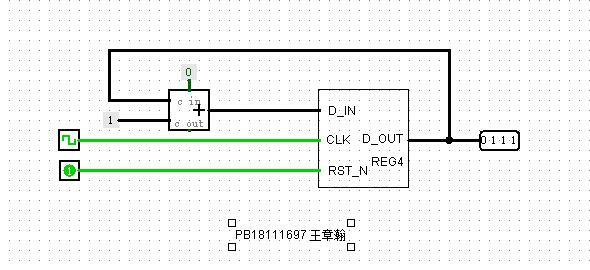
\includegraphics[width=1\linewidth]{step6_counter.jpg}
		\label{step6_counter}
	\end{figure}
	其Verilog代码如下:
	\begin{lstlisting}[language=Verilog]
	module counter(
		input CLK, RST_N,
		output reg [3:0] CNT = 0
		);
		always @(posedge CLK)
		begin
			if(RST_N == 0)
				CNT <= 4'b0;
			else
				CNT <= CNT + 4'b1;
		end
	endmodule
	\end{lstlisting}
	通过Vivado仿真,得到如下波形图:
	\begin{figure}[H]
		\centering
		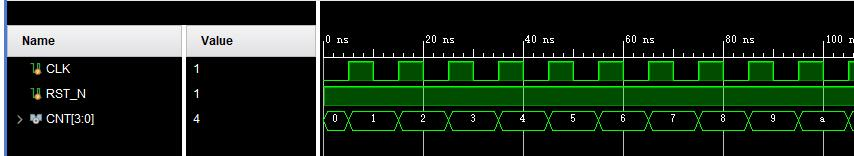
\includegraphics[width=1\linewidth]{step6_Verilog_Simulation.jpg}
		\label{step6_Verilog_Simulation}
	\end{figure}
	
	
	
	\section{实验练习}
	\subsection{题目1}
	在 Logisim 中用与非门搭建 SR 锁存器,画出电路图,并分析其行为特性,列出电路在不同输入时的状态。\par
	\begin{figure}[H]
		\centering
		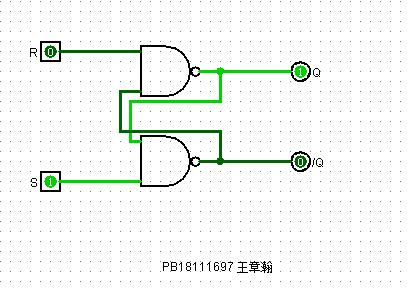
\includegraphics[width=1\linewidth]{p1_SR_Letch_NAND.jpg}
		\label{p1_SR_Letch_NAND}
	\end{figure}
	该电路的行为特性描述如下:当S,R=1,0时,Q置1;当S,R=0,1时,Q置0;当S,R=1,1时,Q保持不变;应当避免S,R=0,0,这是未定义状态。\par
	电路在不同输入时的状态如下表所示:\par
	\begin{tabular}{|c|c|c|c|c|}
		\hline 
		\rule[-1ex]{0pt}{2.5ex} S & R & Q & $\overline{Q}$ & 功能 \\ 
		\hline 
		\rule[-1ex]{0pt}{2.5ex} 0 & 0 & 1 & 1 & 未定义状态 \\ 
		\hline 
		\rule[-1ex]{0pt}{2.5ex} 0 & 1 & 0 & 1 & 置0 \\ 
		\hline 
		\rule[-1ex]{0pt}{2.5ex} 1 & 0 & 1 & 0 & 置1 \\ 
		\hline 
		\rule[-1ex]{0pt}{2.5ex} 1 & 1 & 不变 & 不变 & 保持 \\ 
		\hline 
	\end{tabular} 


	\subsection{题目2}
	在 Logisim 中搭建一个支持同步置位功能的 D 触发器,画出其电路图,并编写对应的 Verilog 代码。\par
	搭建结果的电路图如下图所示:
	\begin{figure}[H]
		\centering
		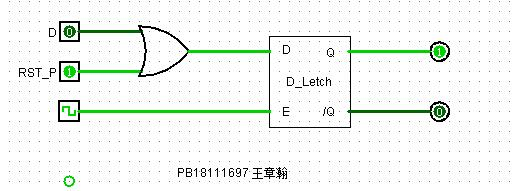
\includegraphics[width=1\linewidth]{e2_circuit.jpg}
		\label{e2_circuit}
	\end{figure}
	其对应的Verilog代码如下:
	\begin{lstlisting}[language=Verilog]
	module D_FF_SYN_RST1(
		input D, CLK, RST_P,
		output reg q
		);
		
		always @(posedge CLK)
		begin
			if(RST_P == 1)
				q <= 1'b1;
			else
				q <= D;
		end
	endmodule
	\end{lstlisting}
	
	
	\subsection{题目3}
	在 Logisim 中搭建一个带有异步复位功能的 D 触发器,画出其完整电路图,并进一步调用该触发器设计一个从 0~15 循环计数的4bit 计数器(可使用 Logisim 中的加法器模块,也可自行设计计数	器) ,写出计数器的 Verilog 代码\par
	搭建结果的电路图如下图所示(各模块中只有带复位的D锁存器较为特殊,故作展示):
	\begin{figure}[H]
	\centering
	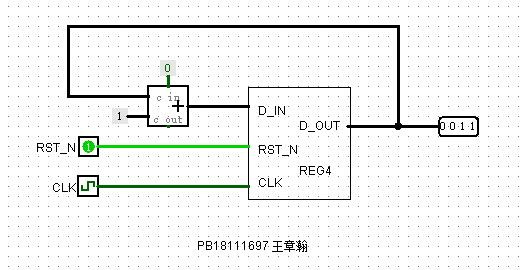
\includegraphics[width=1\linewidth]{e3_counter.jpg}
	\caption{总体电路}
	\label{e3_counter}
	\end{figure}
	
	\begin{figure}[H]
		\centering
		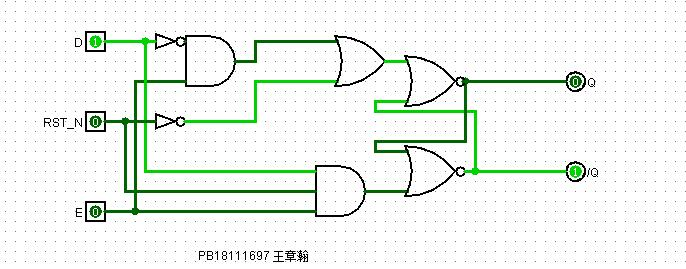
\includegraphics[width=1\linewidth]{e3_D_Letch.jpg}
		\caption{最底层的D锁存器}
		\label{e3_D_Letch}
	\end{figure}

	其对应的Verilog代码如下:
	\begin{lstlisting}[language = Verilog, name=D触发器]
		module D_FF_ASYN_RSTN(
			input d, CLK, RST_N,
			output reg q
			);
			
			always@(posedge CLK or negedge RST_N)
			begin
				if(RST_N==0)
					q <= 1'b0;
				else
					q <= d;
			end
		endmodule
	\end{lstlisting}
	
	
	\begin{lstlisting}[language = Verilog, name=4bit寄存器]
	module REG4(
		input [3:0] D_IN,
		input CLK, RST_N,
		output wire[3:0] D_OUT
		);
		
		D_FF_ASYN_RSTN D_FF_inst0(D_IN[0], CLK, RST_N, D_OUT[0]);
		D_FF_ASYN_RSTN D_FF_inst1(D_IN[1], CLK, RST_N, D_OUT[1]);
		D_FF_ASYN_RSTN D_FF_inst2(D_IN[2], CLK, RST_N, D_OUT[2]);
		D_FF_ASYN_RSTN D_FF_inst3(D_IN[3], CLK, RST_N, D_OUT[3]);
	endmodule
	\end{lstlisting}
	
	\begin{lstlisting}[language = Verilog, name=向上0到15计数]
		module counter_up(
			output[3:0] c);
			reg CLK;
			reg RST_N = 0;
			reg [3:0] num = 4'b0000;
			
			REG4 REG4_init0(num, CLK, RST_N, c);
			
			always
			begin
				RST_N = 1;
				CLK = 0; #5; 
				CLK = 1; #5;
				num = c + 1;
			end
		endmodule
	\end{lstlisting}



	\subsection{题目4}
	在 Logisim 中搭建一个 9~0 循环递减的计数器,复位值为 9,每个周期减一(可使用 Logisim 中的减法器模块,也可自行设计计数器) , 画出电路图,进行正确性测试,并写出其对应的 Verilog 代码。\par
	搭建结果的电路图如下图所示,
	\begin{figure}[H]
		\centering
		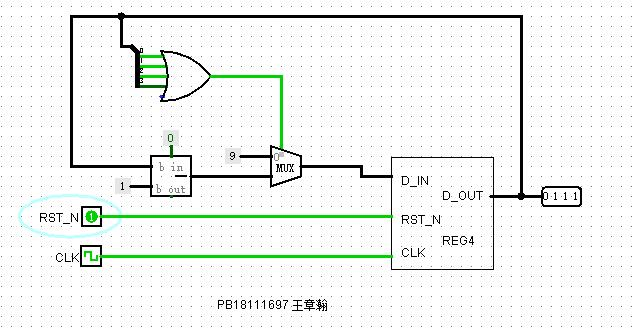
\includegraphics[width=1\linewidth]{e4_counter.jpg}
		\label{e4_counter}
	\end{figure}
	
	
	其对应的Verilog代码如下(只展示与题目3不同的代码部分):
	\begin{lstlisting}[language = Verilog, name=向下9到0计数]
	module counter_down(
		output[3:0] c);
		reg CLK;
		reg RST_N = 0;
		reg [3:0] num = 4'b0000;
		
		REG4 REG4_init0(num, CLK, RST_N, c);
		
		always
		begin
			RST_N = 1;
			CLK = 0; #5; 
			CLK = 1; #5;
			if(num == 0)
				num = 9;
			else
				num = c - 1;
		end
	endmodule
	\end{lstlisting}
	
	
	
	\subsection{题目5}
	前面所有电路的复位信号都是低电平有效,如要使复位信号高电平有效,应如何实现?试用 Logisim 画出一个示例电路,并编写	Verilog 代码。\par
	选取题目4进行修改。\par
	修改的部分的电路图如下:
	\begin{figure}[H]
		\centering
		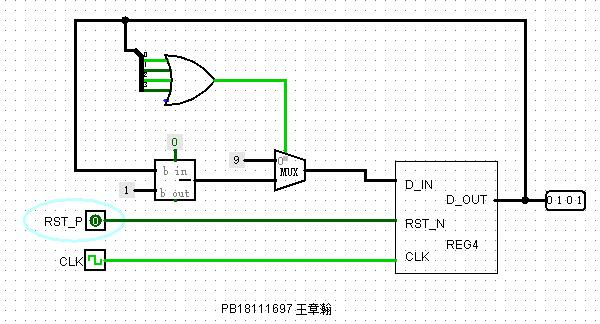
\includegraphics[width=1\linewidth]{e5_counter.jpg}
		\label{e5_counter}
	\end{figure}
	
	而程序相较于题目4只需做如下修改。
	\begin{lstlisting}[language = Verilog, name=向下9到0计数(RST高电平有效)]
	module D_FF_ASYN_RSTP(
	input d, CLK, RST_P,
	output reg q
	);
	
	always@(posedge CLK or posedge RST_P)
	begin
	if(RST_P==0)
	q <= 1'b0;
	else
	q <= d;
	end
	endmodule
	\end{lstlisting}
	
	
	\section{总结与思考}
	
	\subsection{本次实验的收获}
	在本次实验中,体验了使用Logisim作时序逻辑电路,并在Vivado中写出对应代码,并仿真模拟来验证。初步理解了时序逻辑电路在Verilog中的表达。\par
	
	\subsection{评价本次实验的难易程度}
	本次实验内容难度适中,基本上是可以自主完成的。\par
	
	\subsection{评价本次实验的任务量}
	本次实验任务量较大,需要课后花费较长时间才能完成。\par
	
	\subsection{为本次实验提供改进建议}
	暂无建议。
	
\end{document}
